%!TEX TS-program = XeLaTeX
%!TEX TS-program = XeLaTeX
\documentclass[11pt]{article}

\usepackage{amssymb}
\usepackage{amsthm}
\usepackage{amsmath}
\usepackage{mathtools}

\usepackage{fancyhdr}
\usepackage{graphicx}
\usepackage[top=3cm, left=2cm, right=2cm, headheight = 90pt]{geometry}
\usepackage{xltxtra}
\usepackage[font=small,labelfont=bf]{caption}

\usepackage{multicol}

\renewcommand{\theenumi}{\alph{enumi}}


\def\leq{\leqslant}
\def\geq{\geqslant}
\def\N{\mathbb N}
\def\R{\mathbb R}
\def\Z{\mathbb Z}
\DeclarePairedDelimiter\set\{\}

\def\prob{}

\theoremstyle{definition}
\newtheorem{problem}{\prob}


\pagestyle{fancy}

%!TEX TS-program = XeLaTeX

\fancyfoot[CE,CO]{}  % this is to remove page numbers (as you might want for single page docs)

%%!TEX TS-program = XeLaTeX
\renewcommand{\figurename}{Attēls}


\fancyhead[C]{{\Large\bf Graphs 1 - Solutions}\\ \date}

\begin{document}

\noindent 
%\emph{\notes}
\filbreak
%1
\begin{problem}
\textit{[Bridges of Königsberg]}

\textbf{Problem}

City of Königsberg is located on both sides of the river Pregel and on two islands. There are seven bridges connecting islands as shown on Figure \ref{fig:sevenBridges}. Leonhard Euler wants to take a walk that would take him across each bridge exactly once. Can he do this? 

\begin{center}
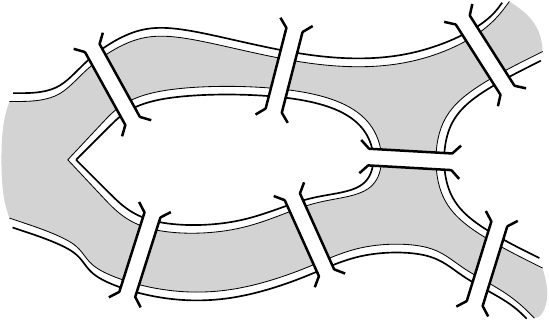
\includegraphics[width=4cm]{euler2.png}
\captionof{figure}{Seven bridges of Königsberg }
\label{fig:sevenBridges}
\end{center} 

\textbf{Solution - Graphs, Vertices, Edges, Paths, Cycles, Power of vertex, Euler's Cycle}

The legend says that this is the actual setting of invention of Graphs. 

What is a graph? Formally, it's a set of \textit{vertices} (usually denoted by $V$) and a set of pairs of vertices - \textit{edges}- denoted by $E$. Luckily, graphs has a nice visual representation - some dots connected by some lines :)

Typical solution of a graph problem looks like - interpret the initial problem as a graph (sometimes trivial, sometimes not), then solve the problem in the graph setting. 

Still some more terminology - a \textit{path} is a sequence of edges such that each starts in the same vertex where previous ends. 

A \textit{cycle} is a path that enters some vertex more than one time, via different edge than the one that it left it. 

A \textit{power of vertex} is number of edges that connects to this vertex.  

\textit{Euler's cycle} is a cycle that contains each edge exactly once. 

So, describing the bridge problem in graph language, its a question if a given graph has an Euler's cycle. 
Some \textit{playing around} gives us impression that it is not possible. 

Indeed the necessary and sufficient condition for existence of Euler's cycle is - all powers of vertices are even (and graph is connected). 

The "necessary" part seems intuitive - since we have to enter each vertex the same amount of times as we exit it, and we have to use different edge every time, then it can not be done if some vertex has an odd power.

The "sufficient" part is a bit more tricky and we shall come back to this in a later lecture (and it makes for good bonus problem!) 
\end{problem}
%
\filbreak
%2
\begin{problem}
\textit{[Weird classmates]}

\textbf{Problem}

A student once told James: "We have $35$ students in our class. And imagine - everyone has exactly $11$ friends within the class!". James, being good at Graph Theory, immediately replied that this is not possible. How did he know?

\textbf{Solution - Property of powers of vertices, double counting}

One popular method of deriving contradictions in combinatorics and, in particular, in graph theory, is called \textit{double counting}. Let's try to apply it to this problem.

Let's try to count the number, or more specifically, the parity of the sum of powers of all edges $S$. One one hand, since we are interested only in the parity, we can ignore all the even powers and express parity of $S$ as number of vertexes with odd powers. 

On the other hand, $S$ can be counted as $2 \times \abs{E}$ (where $E$ is a set of edges), because each edge has exactly two ends and sum of all ends of edges equals the sum of powers of all vertices. 

From this second way of counting we see that $S$ is always even, therefore, from first way of counting, number of vertices with odd powers are even!
\end{problem}
%
\filbreak
%3
\begin{problem}
\textit{[Road planning]}

\textbf{Problem}

In the Kingdom of Wakanda there are $15$ towns and each of these are connected with direct roads with no less than $7$ other towns within this Kingdom. Prove that its possible to travel by road between any two towns (possibly via other towns)!

\textbf{Solution - contradiction in graphs}

Let's assume the opposite - there are towns $a$ and $b$ that are not connected - there is no path that connects them.  By $A$ and $B$ we shall denote the sets of vertices that are directly connected to $a$ and $b$ respectively. If these sets were intersecting, say, $c \in A$ and $c \in B$ then there would exist a path $a-c-b$, which is a contradiction to our assumption. 
However, if $A \cap B$ is empty, then, if we count the vertices we have to put in the disjoints sets $\set{a}; A; B; \set{b}$, and recalling that by given $\abs{A} \ge 7$ and $\abs{B} \ge 7$, we get $1 + 7 + 7 + 1 = 16$ which is greater than number of vertices we have - $15$. Therefore, we again arrive at contradiction,  and it must be that $a$ and $b$ are connected.

This is a particular case of a general sufficient (but not necessary) condition for a graph to be connected: minimum power of vertex has to be at least $\floor{\frac{\abs{V}}{2}}+1$

It is an easy exercise to prove it in a general form!
\end{problem}
%
\filbreak
%4
\begin{problem}
\textit{[Wire cube]}

\textbf{Problem}

Luize has a $120cm$ long piece of wire.
\begin{enumerate}
\item Can she make a cube with side length $10cm$ without cutting the wire?
\item If she does need to cut it, what is the minimum number of pieces?
\end{enumerate}

\textbf{Solution - Euler's path}

First let's observe that a cube has $12$ edges and is we want a cube with height $10cm$ then we need $120cm$ of wire. For Luize this means that she can not run wire on any side more than once. 
This allow us to reformulate the problem into graph language - does this graph have an Euler's path. 

\textit{Euler's path} similarly to Euler's cycle, is a path that contains all the edges exactly once (but does not have to end in the starting vertex.

Turns out the necessary and sufficient condition for existence of Euler's path is: in a connected graph there are exactly $0$ or $2$ vertices with odd power. 

Our graph (the skeleton of cube) has $8$ vertices with odd powers, therefore first part is impossible. 

If there are $2$ vertices with odd powers in a connected graph, then Euler's path starts at one of them and ends at the other. This means that every piece of wire Luize wants to use has to start at one vertex of a cube and end at another and each vertex has to have at least one end of one piece. Therefore, Luize will have to cut wire into at least $4$ parts.

\end{problem}
%
\filbreak
%5
\begin{problem}
\textit{[Doodle]}

\textbf{Problem}

Is it possible to draw the picture from the Figure \ref{fig:doodle} without lifting pen from the paper?
\begin{center}
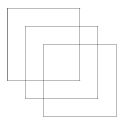
\includegraphics[width=3cm]{doodle.png}
\captionof{figure}{A doodle }
\label{fig:doodle}
\end{center} 

\textbf{Solution - Euler's path}

This again can be viewed as a question of existence of an Euler's cycle in a graph. In this case all the vertices (cross-points) have even powers, therefore it is possible (and it is easy to show an example).
\end{problem}
%
\filbreak
%6
\begin{problem}
\textit{[Types of tournament]}

\textbf{Problem}

30 teams participated in the tournament. What was the total number of games they played, if:
\begin{enumerate}
\item All teams have to play each other
\item They do play-offs (in each game loser goes out, winner moves to next stage)
\end{enumerate}

\textbf{Solution - Size of full graphs, size of trees}

A graph where every two vertices are connected by an edge is called a \textit{full graph}. A tournament where  every team plays every other, can be seen as a full graph. 

So - how do you count the number of edges in a full graph with $n$ vertices? One way of thinking about it - each of $n$ vertices has an outgoing edge to each of $n-1$ remaining vertices, but this way we have counted each edge twice (one time from each end). Therefore, number of edges in an full edge is $\frac{n(n-1)}{2}$ 

Now, the playoffs ... this tournament can also be represented by a graph, but not a full one. It is, in fact, a \textit{tree}, but more on those later. How many edges would this graph has? We can count them in a following way - as a result of every game, exactly one team leaves tournament. Tournament starts with $n$ teams, and stops when there is only $1$ team left. Therefore, exactly $n-1$ games have happened!
\end{problem}
%
\filbreak
%7
\begin{problem}
\textit{[Circular reference]}

\textbf{Problem}

Edges of a regular polygon are marked with arrows (in one of the two possible directions). Prove that number of vertices which have two arrows going out of them is equal to number of vertices which have two arrows going into them!

\textbf{Solution - Double counting}

Say the polygon has $n$ edges, and therefore $n$ arrows.
Now we count the number of vertexes in two ways. 
First (directly), number of vertexes is equal to the number of edges, hence $n$.
On the other hand, there are three types of vertices only - 
\begin{itemize}
\item Vertices where two arrows meet. We denote number of these by $k$.  Note that out of $n$ arrows, $2k$ enter into these vertices.
\item Vertices where only one arrow enters. Since all the remaining arrows have to enter these and there are $n - 2k$ arrows left, then there are exactly $n - 2k$ such vertices.  
\item Vertices where no arrow enters. Now, if we count how many are left, we get $n - k - (n -2k) = k$ and we see that we have proven the problem! 
\end{itemize}


\end{problem}
%
\filbreak
%8
\begin{problem}
\textit{[Forestry]}

\textbf{Problem}

A \textit{tree} is a set of nodes connected by sticks (each stick connecting exactly two nodes) where it is possible to travel between any two nodes (graph is connected), but it is not possible to travel somewhere and come back to original node not going though same stick twice (graph has no cycles).  A leaf is a node with just one stick connecting it. Prove that every tree has at least two leaves!

\textbf{Solution - Extreme Element}

Sketch of the solution: we consider the longest path in this graph and show that there has to be a leaf on each end of it.

Start with a method called \textit{Extreme Element} - we choose some element with a maximum (or minimum property) and then work from there. In this case, since tree by definition does not have any cycles, there has to exist a longest path (or, if several such exist, we choose one of them). Denote this path $A$ with $A_1,A_2,\dots A_n$.

Now a question - can there be another edge from $A_1$ (besides one going to $A_2$? If there is such an edge $e$, there can be only two options:
\begin{itemize}
\item $e$ goes to some $A_i$ that belongs to $A$, $i \ne 2$. This is contradicting the fact that a tree contains no cycles, because $A_1, A_2, \dots, A_i$ would form a cycle. 
\item $e$ goes to some $B_1$ that does not belong to the $A$. This, however is a contradiction to the property of our extreme element - the fact that $A$ is of maximum length - because clearly there exists a path $B = B_1,A_1,A_2,\dots A_n$ that is longer than $A$!
\end{itemize}
We have shown contradictions in all possible cases and therefore there can be no other edge leaving $A_1$. Therefore $A_1$ is a leaf. 

Following exactly the same argument we can prove that $A_n$ also has to be a leaf, and we are done - every tree has at least two leaves. 

\end{problem}
%
\filbreak
%9
\begin{problem}
\textit{[Network robustness]}

\textbf{Problem}

What is the minimum number between of connections between $10$ information nodes to guarantee that if any two of them break down, the rest are still connected? 

\textbf{Solution - Example construction}

First we show that each node has to have at least $3$ connections. Indeed that is easy to see, because if there was a node $A$ with only two connections, say, to $B$ and $C$ then if $B$ and $C$ break down then $A$ would get disconnected from the rest.

Therefore there has to be at least $10\times 3 \div 2 = 15$ connections - $3$ leaving each of $10$ nodes, but then we have counted each connection twice. 

Interestingly, it is rather non trivial to show an example with $15$ edges that works and convince reader that it works. 

The example (Fig. \ref{fig:double5}) consists of two pentagons - $A=A_1,\dots, A_5$ and $B=B_1,\dots,B_5$ and all pairs $(A_i;B_i)$ are connected.
\begin{center}
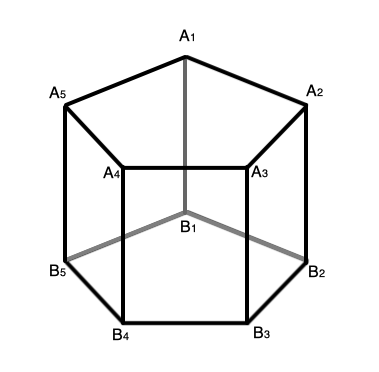
\includegraphics[width=5cm]{double5.png}
\captionof{figure}{A robust network}
\label{fig:double5}
\end{center} 

Now, why does this work? 
If the two nodes break down, there are two possibilities:
\begin{itemize}
\item Both nodes belong to one pentagon, say $A$. Nodes in $A$ can now be disconnected within $A$, but they are all still connected to their corresponding nodes in $B$, and $B$ is intact and connected, so all nodes are still connected.
\item Broken nodes are in different pentagons (one in $A$ and one in $B$). It is easy to see that no matter which node you remove, remaining $4$ nodes in each pentagon are still connected. On the other hand, there are still at least $3$ pairs $(A_j;B_j)$ such that both $A_j$ and $B_j$ are not broken, therefore the remaining pentagon parts will still be connected to each other.
\end{itemize}

\end{problem}
%
\filbreak

\end{document}
